
% Trabalhos Relacionados
%

\chapter{Trabalhos Relacionados}
\label{Chapter:RelatedWork}

Neste capítulo serão apresentados modelos, ferramentas e metodologia utilizados
para apoiar profissionais nas atividades de desenvolvimento, manutenção e
evolução de software. Serão apresentadas as ferramentas comumente utilizadas ---
como \textit{loggers}, depuradores e \textit{profilers} ---, trabalhos inseridos
nas áreas de Cognição, Compreensão e Visualização de Software, bem como
trabalhos onde a análise dos sistemas de software é feita por meio da Teoria de
Redes Complexas.

\section{\textit{Loggers}, Depuradores e \textit{Profilers}}
\label{sec:Loggers}

\textit{Loggers} são ferramentas que monitoram a execução de sistemas de
software através de registros ou entradas de \textit{log}.
Os registros podem estar dispostos em um formato específico ---
\textit{extensible markup language} (XML), \textit{JavaScript Object Notation} (JSON),
entre outros --- ou constar como texto informativo.
Podem ainda estar associados a níveis distintos --- \textit{information},
\textit{warning}, \textit{error}, entre outros.
As informações podem ser veiculadas a diferentes tipos de mídia, como arquivos
texto, arquivos binários, bases de dados relacionais, não relacionais ou
armazenadas em memória.

A análise de um conjunto de registros usualmente se dá por cálculos estatísticos
e por meio de mecanismos de buscas convencionais na mídia nos quais eles foram
veiculados.
Tais ferramentas possuem diferentes métodos de entradas. Seus recursos podem ser
acessados através de um protocolo específico, de uma
\textit{application program interface} (API) ou de funções e métodos.
São exemplos de \textit{loggers}:
SmartInspect\footnote{Disponível em: \href{http://www.gurock.com/smartinspect/}{http://www.gurock.com/smartinspect/}. Acessado em 18/05/2017.},
Logentries\footnote{Disponível em: \href{http://logentries.com/}{http://logentries.com/}. Acessado em 18/05/2017.} e
Logentries\footnote{Disponível em: \href{http://sentry.io/welcome/}{http://sentry.io/welcome/}. Acessado em 18/05/2017.}.

%\section{Depuradores}
%\label{sec:Debuggers}

Depuradores são ferramentas que possibilitam avaliar a execução de sistemas de
software. Tais ferramentas permitem definir pontos de parada ---
\textit{breakpoints}, \textit{watchpoints} e \textit{catchpoints} ---,
condicionais ou não, nos quais o depurador pausa a execução. Uma vez pausada a
execução do sistema, pode-se executar até o próximo ponto de parada, próxima
expressão, ou adentrar uma definição --- como um método ou função. Permitem ainda
avaliar determinadas expressões e monitorar certos valores de variáveis do
sistema.

Alguns depuradores implementam funcionalidades que permitem a depuração de:
sistemas já em execução; software em execução em máquina remota; programas
\textit{multithread}. Outras funcionalidades e técnicas de depuração são
disponibilizadas por depuradores e desenvolvidas por pesquisadores.
\citeonline{Engblom:ReverseDebuggin:2012} revisou o estado da arte referente à
depuração reversa, que consiste em interromper a execução do software ao se
constatar uma falha e desfazer o histórico de execuções para se avaliar o que a
causou.
São exemplos de depuradores \textit{The GNU Project Debugger} (GDB)
\footnote{Disponível em: \href{http://www.gnu.org/s/gdb/}{http://www.gnu.org/s/gdb/}. Acessado em 18/05/2017.} e 
\textit{The Java Debugger} (JDB)
\footnote{Verifique: \href{http://www.tutorialspoint.com/jdb/}{http://www.tutorialspoint.com/jdb/}. Acessado em 18/05/2017.}.

%\section{\textit{Profilers}}
%\label{sec:Profilers}

\textit{Profilers} são ferramentar utilizadas para extrair dados da execução de
sistemas de software através de técnicas de análise estática e dinâmica.
\citeonline{Thiel:2006:Profiling} analisa 8 ferramentas e discorre sobre
instrumentação em tempo de compilação, ferramentas de amostragem, instrumentação
através de contadores de hardware, instrumentação binária, dentre outras
técnicas.
São exemplos de ferramentas de \textit{profiling} Gprof\footnote{Verifique: \href{https://sourceware.org/binutils/docs/gprof/}{https://sourceware.org/binutils/docs/gprof/}. Acessado em 20/05/2017}
e Dtrace\footnote{Verifique: \href{http://dtrace.org/blogs/about/}{http://dtrace.org/blogs/about/}. Acessado em 20/05/2017}.

\citeonline{Henderson:2017:Software} relatou as principais práticas de
Engenharia de Software praticadas pela empresa Google\footnote{Disponível em:
\href{http://www.google.com/}{http://www.google.com/}. Acessado em 20/05/2012}.
Na seção referente às ferramentas de depuração e \textit{profiling}, Henderson
constata que os servidores da empresa possuem bibliotecas que disponibilizam
determindas ferramentas de análise. No caso de falha, informações da execução do
serviço --- amostradas, em alguns casos --- são salvas em arquivos de
\textit{log}. Menciona ainda sobre uma interface web para depurar 
\textit{remote procedure calls} (RCPs), alterar argumentos de linha de comando,
avaliar uso de recursos computacionais, \textit{profiling}, entre outras coisas.
Discorre brevemente, por fim, da facilidade de se depurar sistemas de software
na empresa e o quão raras são as ocasiões em que se mostra necessário utilizar
um depurador convencional como o GDB.

O modelo proposto neste trabalho irá registrar trilhas de execução em
\textit{log}. A instrumentação do sistema de software estudado pode ser
contínua ou desabilitada --- até mesmo amostrada. A integração do modelo com
a execução do sistema em tempo real não foi considerada, embora tecnicamente
possível. Isso viabilizaria, por exemplo, uma técnica de depuração através da
rede do software.

\section{Cognição, Compreensão e Visualização de Software}
\label{sec:SoftwareCognition}

\citeonline{Pacione:2004:Software} teorizou um modelo com três dimensões de
abstração.
A primeira dimensão trata da granularidade dos elementos de tal
modelo: em um nível de menor granularidade são consideradas as instruções e
expressões; componentes e pacotes representam um nível maior de granularidade.
A segunda dimensão trata das diversas facetas pelos quais os componentes podem
ser avaliados, como por exemplo a análise da estrutura do software, de seu 
comportamento ou do fluxo de dados.
A terceira dimensão trata do tipo de análise empregada, se estática ou dinâmica.
\citeonline{Pacione:2004:NovelModel} criou um modelo com base no modelo
teorizado por \citeonline{Pacione:2004:Software}.

A granularidade selecionada para análise não é necessariamente homogênea no
modelo proposto neste trabalho: enquanto parte do sistema é considerada em nível
maior granularidade, outras partes da rede podem ser expostas de forma
detalhada. Cada componente da rede remete a um ou mais elementos da estrutura
estática do software, enquanto que as ligações revelam as interações entre esses
componentes durante a execução do sistema. O fluxo de dados pode ser
parcialmente observado ao passo em que essas interações ocorrem, uma vez que o
modelo, a priori, não provê mecanismos de monitorar valores.

\citeonline{Hendrix:2002:ControlStructureDiagrams} propos diagramas de
estruturas de controle (Figura \ref{Figure:ControlStructureDiagram})
renderizados juntamente com o código-fonte no editor de texto e validou a
eficácia de tais diagramas através de dois experimentos, com 38 e 50 estudantes.
Os estudantes foram separados em dois grupos --- controle e experimental --- com
o mesmo número de indivíduos, para cada experimento.
A análise estatística rejeitou fortemente a hipótese nula do estudo que
considera não relevante que diagramas de estruturas de controle afetam
positivamente a performance dos entrevistados em responderem perguntas.

\begin{figure}[!htb]
    \centering
    \caption{Diagramas de Estruturas de Controle}
    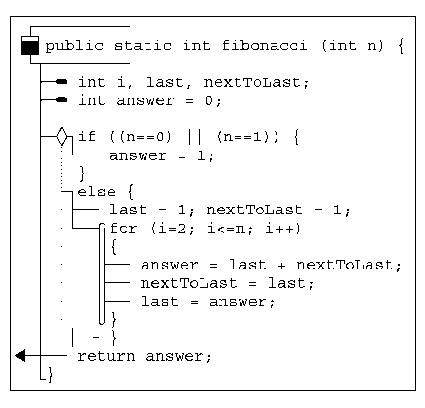
\includegraphics[scale=1.4]{../shared files/figures/2.02....related...work/control structure diagram.pdf}
    \fonte{\citeonline{Hendrix:2002:ControlStructureDiagrams}}
    \label{Figure:ControlStructureDiagram}
\end{figure}

\citeonline{roach2011using} estudaram sistemas de software do ponto de vista da 
teoria de redes complexas e alteraram propriedades visuais da rede referente ao
sistema Python (Figura \ref{Figure:PythonNetworks}) com o intuito de destacar a
correlação entre número de erros (primeiro grafo) e o número de desenvolvedores
(segundo grafo) por arquivo.

\begin{figure}[!htb]
    \centering
    \caption{Mapa de calor aplicado às redes referentes ao sistema Python}
    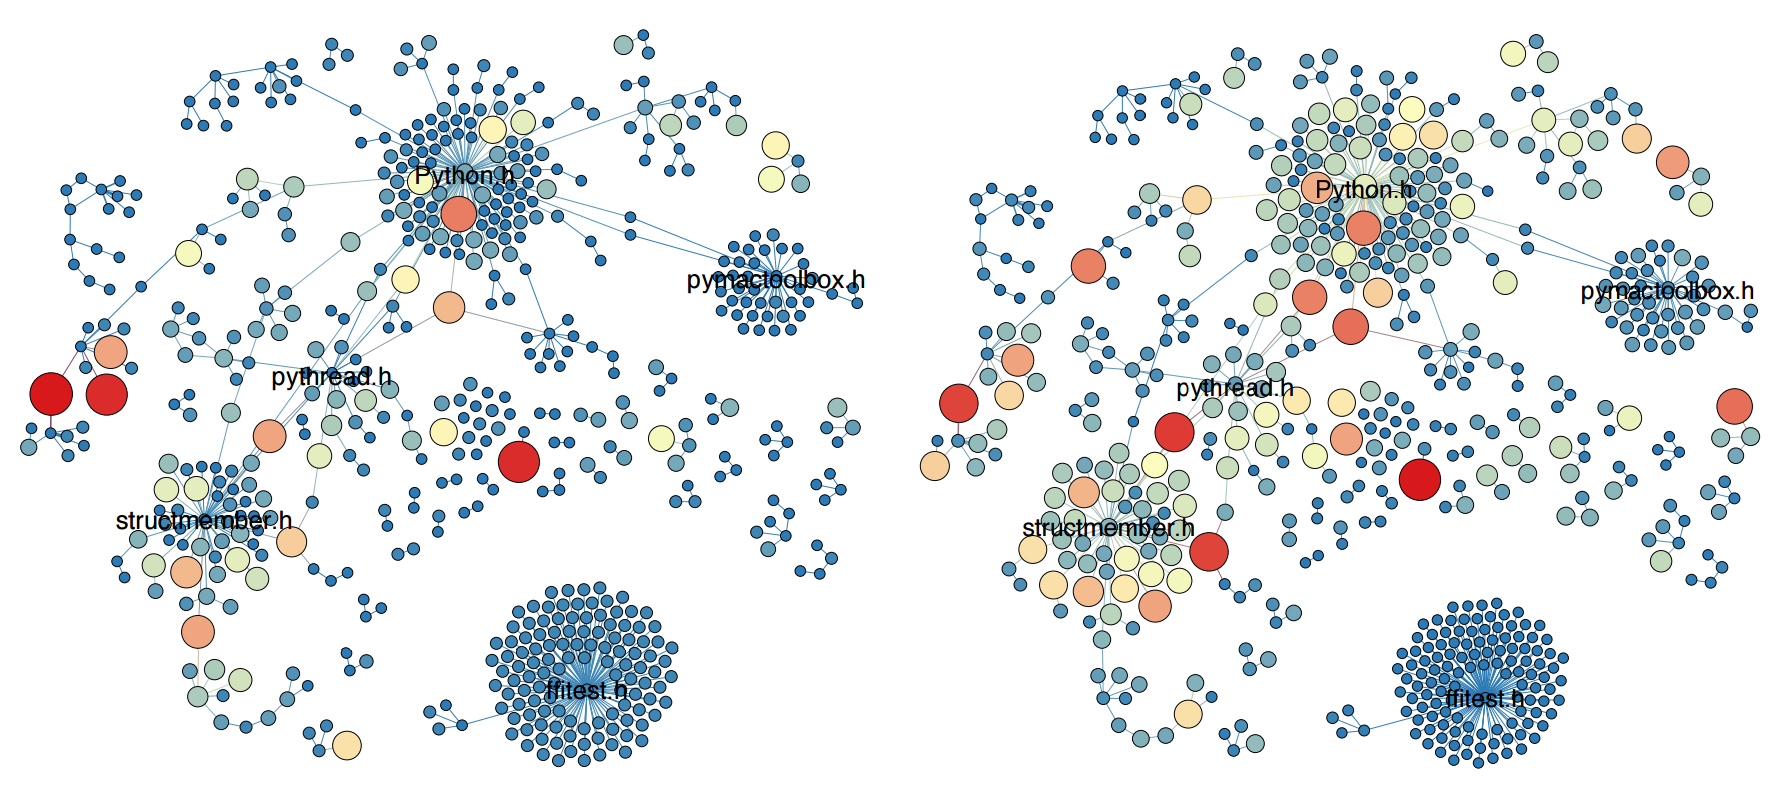
\includegraphics[width=1\textwidth]{../shared files/figures/2.02....related...work/PythonNetworks.png}
    \fonte{\citeonline{roach2011using}}
    \label{Figure:PythonNetworks}
\end{figure}

O destaque ou ocultação visual de certas informações pode auxiliar na
compreensão de redes da estrutura de execução de sistemas de software e suas
propriedades.

\citeonline{kim2011crash} aborda um problema de Qualidade na área da Engenharia
de Software sobre triagem de defeitos. Parte do trablaho consiste na coleta e
tratamento de trilhas de execução que resultam em defeitos para a construção de 
um grafo através de um processo de decomposição e agregação. Tal técnica é
inspirada no trabalho de \citeonline{jeong2009improving} e é idêntica ao
operador de redução espacial $\mathcal{S}$ utilizado nesta dissertação.

Esta dissertação propõe a análise de sistemas de software por técnicas híbridas,
onde ora consideramos aspectos dinâmicos, ora estáticos.
Uma vez que a maior parcela de trabalhos citados neste capítulo utiliza de
análise estática para a aquisição de dados, se faz necessário destacar trabalhos
que usam de análise dinâmica ou híbrida.

\citeonline{alimadadi2014understanding} implementaram ferramenta que captura
eventos e exibe: uma visão geral de tais eventos em determinado contexto;
detalhes de um evento enquanto mantém referência na linha de eventos; por fim,
todas informações capturadas de um determinado evento.
\citeonline{alimadadi2016understanding} disponibilizaram ferramenta que
instrumenta execuções assíncronas em aplicações JavaScript \textit{full-stack},
de forma que mantém relações temporais e contextuais entre código executado em
máquina cliente e servidor.

\citeonline{fittkau2017software} codificaram ferramenta que mapeia aplicações
através de infra-estrutura em núvem, bem como instrumenta aplicações em execução
e constrõem \textit{treemaps} com arestas entre componentes comunicantes.

\citeonline{jayaraman2017compact} representam a execução de sistemas Java
através de adaptações de diagramas de objetos e diagramas de sequência.
Tais diagramas --- originários da \textit{unified modeling language} (UML) ---
sofrem, segundo os autores, compressões verticais e horizontais, de forma a
reduzir a quantidade de informação neles contida.
\citeonline{muhammad2017visualizing} propuseram a visualização de trilhas de
execução instrumentadas do \textit{bytecode} das APIs de coleções de Java
através de \textit{treemaps}. 

\citeonline{ezzati2017multi} rrevisa literatura acerca da representação e
navegação de grandes volumes de trilhas de execução. Esta dissertação faz uso de
todas as técnicas baseadas no conteúdo de trilhas de execução: redução,
generalização, agregação e agrupamento. A técnica de visualização adotada neste
trabalho é multinível e hierárquica, ao passo em que apresenta o modelo de forma
a preencher o espaço disponível para tal.

\section{Análise de Software por Redes Complexas}
\label{sec:SoftwareComplexNetworks}

Todos os trabalhos que tratam da análise de software por redes complexas citados
nesta seção apontam que tais redes apresentam propriedades de redes de mundo
pequeno e livres de escala, despeito da diferenças tecnológicas dos sistemas em
análise e metodológicas no que se refere à construção de tais redes, isto é, o
que são seus elementos e o que representam as ligações entre eles.

% primeiro trabalho
\citeonline{Valverde:2002:Complex} foram os pioneiros ao introduzir a Teoria de
Redes Complexas à análise de sistemas de software, pois modelaram uma rede com
ligações não direcionadas entre classes. O trabalho analisou dois sistemas:
\textit{Java Development Framework} 1.2 e \textit{UbiSoft ProRally 2002}.
Os autores constataram que os sistemas apresentam propriedades de redes de mundo
pequeno e de redes livres de escala através de processos locais de otimização
--- no lugar das regras de anexação preferencial, teorizadas por
\citeonline{Barabasi:1999:EmergenceScaling}, ou de duplicação-reconexão,
teorizadas por \citeonline{Alexei:2003:ModelingProtein}.

% arestas direcionadas, múltiplas tecnologias
\citeonline{Myers:2003:Complex} argumentou que a natureza da relação entre
componentes altera o fluxo de dados e é, portanto, significante, de modo que a
rede modelada deve conter ligações direcionadas entre seus nós. Este trabalho
estudou 3 sistemas orientados a objetos e outros 3 sistemas procedurais através
de grafos de colaboração obtidos por análise estática.

Faz-se necessário destacar que a metodologia para a construção das redes não é 
única: são distintas nos trabalhos de \citeonline{Myers:2003:Complex} e de 
\citeonline{Valverde:2002:Complex} não somente pelo direcionamento ou não de
ligações, mas do que constitui os elementos das redes e o que representam as
ligações entre eles. Trata-se de um processo de modelagem, portanto.

% hierarquia: arquivos de cabeçalho
Alguns trabalhos modelam as redes de forma homogênea em determinado nível
hierárquico --- métodos, classes, arquivos de cabeçalhos, pacotes, entre outros.
\citeonline{Moura:2003:Signatures} analisou rede formada por cabeçalhos de
sistemas escritos em \texttt{C} e \texttt{C++}.
Apontam ainda que o crescimento do sistema é o processo que faz com que a rede
seja livre de escala --- processo de anexação preferencial, conforme destacado
por \citeonline{Barabasi:1999:EmergenceScaling} ---, enquanto que o processo de
manutenção perfectiva é responsável pela configuração da rede de mundo pequeno.
% hierarquia: pacotes
\citeonline{LaBelle:2004:PackageNetworks}, por sua vez, estudaram a rede de
dependências entre pacotes dos repositórios Debian GNU/Linux e FreeBSD Ports
Collection.

% hierarquia: múltiplos níveis separadamente
Certos trabalhos fazem relação entre redes distintas em diferentes
níveis hierárquicos, mas ainda homogêneas, como o trablaho de
\citeonline{Carneiro2013sourceminer}. Embora não abordem diretamente a teoria de
redes complexas.
% hierarquia: múltiplos níveis conjuntamente
\citeonline{pan2011multi} propuseram redes em múltiplos níveis de granularidade,
onde uma rede construída contém conjuntamente elementos da estrutura de pacotes,
classes e métodos.

% peso nas redes
\citeonline{ma2010hybrid} valora ligações e elementos das redes estudas de
acordo com métricas de software. \citeonline{chong2015analyzing} valora as
ligações entre elementos das redes de acordo com seu tipo (agregação,
composição, depedência, entre outros) e dos componentes em questão, cuja
complexidade varia de acordo com métricas de software. Não valora os elementos
da rede, no entanto.
